\documentclass[12pt, a4paper]{article}
\usepackage[T2A]{fontenc}
\usepackage[utf8]{inputenc}
\usepackage[russian]{babel}
\usepackage{graphicx}
\usepackage{amsfonts}
\usepackage{indentfirst}
\usepackage{amsmath}
\usepackage{amsthm}
\usepackage{nicematrix}
\usepackage{hyperref}
\hypersetup{
    colorlinks=true,
    linkcolor=black,
    filecolor=magenta,      
    urlcolor=cyan,
    pdftitle={Lab4},
    pdfpagemode=FullScreen,
}
\usepackage{soulutf8}
\usepackage[left=1cm,right=1cm,
    top=2cm,bottom=2cm]{geometry}
\usepackage{titleps}
    \newpagestyle{main}{
        \setheadrule{0.4pt}
        \sethead{something}{\thepage}{}
}
\usepackage{listings}
\usepackage{color}

\definecolor{dkgreen}{rgb}{0,0.6,0}
\definecolor{gray}{rgb}{0.5,0.5,0.5}
\definecolor{mauve}{rgb}{0.58,0,0.82}

\lstset{frame=tb,
  language=Python,
  aboveskip=3mm,
  belowskip=3mm,
  showstringspaces=false,
  columns=flexible,
  basicstyle={\small\ttfamily},
  numbers=none,
  numberstyle=\tiny\color{gray},
  keywordstyle=\color{blue},
  commentstyle=\color{dkgreen},
  stringstyle=\color{mauve},
  breaklines=true,
  breakatwhitespace=true,
  tabsize=3
}
%\pagestyle{main}
\theoremstyle{plain}
\newtheorem{theorem}{Теорема}[section]
\newtheorem{corollary}{Следствие}[theorem]
\newtheorem*{example}{\textit{Пример}}
\newtheorem*{definition}{Определение}
\begin{document}
\begin{titlepage}
    \newpage
    \begin{center}
        \begin{tabular}{cc}
            \parbox{12cm}{\centering \textbf{НИУ ИТМО}} \\
            \\
            \hline
            \hline
        \end{tabular}
    \end{center}

    \begin{center}
        \caps{\textbf{Факультет систем управления и робототехники}}\\
    \end{center}

    \vspace{1cm}

    \begin{center}
        \textsc{Лабораторная работа №6 \\ по дисциплине <<Частотные методы>>}
    \end{center}

    \vspace{8em}

    \noindent Выполнил:  \hfill Гридусов Д.Д

    \vspace{20pt}
    \noindent Преподаватель: \hfill Перегудин А.А \\
    \\
    \vfill
    \begin{center}
        Санкт-Петербург \\2024 г.
    \end{center}

\end{titlepage}

\tableofcontents
\newpage

\section{Фильтрация изображений с переодичностью}
\noindent Загрузим изображение в Matlab, переведем его в формат double в диапазоне от 0 до 1.
\noindent С помощью встроенных функций построим образ Фурье, поделим его на модуль и агумент и выведем получившиеся изображения: 
\begin{figure}[!htb]
    \minipage{0.5\textwidth}
    \includegraphics[width=\linewidth]{../image/part-1/fourier_img_argument.png}
    \caption{Аргумент образа Фурье}
    \endminipage\hfill
    \minipage{0.5\textwidth}
    \includegraphics[width=\linewidth]{../image/part-1/fourier_orig_version.png}   
    \caption{Модуль образа Фурье}
    \endminipage\hfill
\end{figure}
\\
\noindent Левое изображение с аргументом образа Фурье нам на данный момент не очень интересно, так как оно пригодится лишь при формировании отфильтрованного изображения.\\
\noindent А вот  модуль мы рассмотрим повнимательнее в поисках "синусных" пиков - как раз они и дают переодичность изображению. Если их замазать, то по идее, наше изображение примет более четкий вид, перестанет быть переодичным.
\noindent Выведем приближенные модули образа Фурье: с незамазанными пиками и с уже замазанными: 
\begin{figure}[!htb]
    \minipage{0.5\textwidth}
    \includegraphics[width=\linewidth]{../image/1_1.jpg}
    \caption{Оригинальный модуль образа Фурье} 
    \endminipage\hfill
    \minipage{0.5\textwidth}
    \includegraphics[width=\linewidth]{../image/1_0.jpg}   
    \caption{Исправленный модуль Фурье-образа}
    \endminipage\hfill
\end{figure}
\newpage 

Проверим гипотезу о том, что переодичность пропадает.
\begin{figure}[!htb]
    \minipage{0.5\textwidth}
    \includegraphics[width=\linewidth]{../image/part-1/15.png}
    \caption{Оригинальное} 
    \endminipage\hfill
    \minipage{0.5\textwidth}
    \includegraphics[width=\linewidth]{../image/part-1/wave_new}   
    \caption{Отфильтрованное изображение}
    \endminipage\hfill
\end{figure}
\section{Размытие изображений}
\noindent Возьмем тоже самое изображение, переведем его черно-белый формат и создадим 3 матрицы блочного размытия с размерностями: $(3\times 3), (21\times 21), (33 \times 33)$.
\begin{figure}[!htb]
    \centering
    \includegraphics[width=0.7\linewidth]{../image/grayImg.png}   
    \caption{Исходное изображение}
\end{figure}
\newpage 

\noindent Применим матрицы к исходному изображению: 
\begin{figure}[!htb]
    \centering
    \includegraphics[width=0.4\linewidth]{../image/img_block_blur1.png}   
    \caption{Блочное размытие, n = 3}
\end{figure}
\newpage 
\begin{figure}[!htb]
    \centering
    \includegraphics[width=0.4\linewidth]{../image/img_block_blur2.png}   
    \caption{Блочное размытие, n = 21}
\end{figure}
\begin{figure}[!htb]
    \centering
    \includegraphics[width=0.4\linewidth]{../image/img_block_blur3.png}   
    \caption{Блочное размытие, n = 33}
\end{figure}

\noindent Перейдем к размытию по Гауссу, заполним 3 матрицы тех же размерностей что и для блочного, и применим к исходному изображению:
\begin{figure}[!htb]
    \centering
    \includegraphics[width=0.4\linewidth]{../image/img_gauss_blur1.png}   
    \caption{Гауссовское размытие, n = 3}
\end{figure}
\newpage 
\begin{figure}[!htb]
    \centering
    \includegraphics[width=0.4\linewidth]{../image/img_gauss_blur2.png}   
    \caption{Гауссовское размытие, n = 21}
\end{figure}
\newpage
\begin{figure}[!htb]
    \centering
    \includegraphics[width=0.4\linewidth]{../image/img_gauss_blur3.png}   
    \caption{Блочное размытие, n = 33}
\end{figure}

\noindent Стоит отметить, что раньше мы пользовались встроенной функцией conv2 для примения фильтров. Теперь воспрользуемся теоремой о свертке (свертка функций равна произведению их образов). Найдем Фурье образ от изображения и от каждого из трех гауссовских ядер, заполнив пропуски нулями. После чего поэлементно перемножим Фурье образ изображения с образом от каждого их фильтров. И возьмем обратное Фурье-преобразование. Выведем результаты размытия: 


\begin{figure}[!htb]
    \centering
    \includegraphics[width=0.4\linewidth]{../image/img_conv1.png}   
    \caption{Гауссовское размытие - теорема о свертке, n = 3}
\end{figure}
\newpage 
\begin{figure}[!htb]
    \centering
    \includegraphics[width=0.4\linewidth]{../image/img_conv2.png}   
    \caption{Гауссовское размытие - теорема о свертке, n = 21}
\end{figure}

\begin{figure}[!htb]
    \centering
    \includegraphics[width=0.4\linewidth]{../image/img_conv3.png}   
    \caption{Блочное размытие - теорема о свертке, n = 33}
\end{figure}
\noindent Видно, что результатыт полученные с помощью свертки и Фурье образов совпали, значит теорема о свертке работает.
\\
\noindent Что касается отличий гауссовского размытия от блочного, гауссовское более плавное и сохраняет больше деталей.
\section{Увеличение резкости}
\noindent Стабильность - признак мастерства, поэтому возьмем то же самое изображение.
\begin{figure}[!htb]
    \centering
    \includegraphics[width=0.4\linewidth]{../image/grayImg.png}   
    \caption{Исходное изображение}
\end{figure}
\newpage
Также зададимся ядром, с помощью которого увелчим резкость изображения:
$$
K
= 
\begin{bmatrix}
    0 & -1 & 0\\
    -1 & 5 & -1\\
    0 & -1 & 0
\end{bmatrix}
$$
Применим с помощью функции Matlab conv2 матрицы ядра к картинке. Посмотрим на результат: 
\begin{figure}[!htb]
    \centering
    \includegraphics[width=0.47\linewidth]{../image/3_s1.png}   
    \caption{Более резкое изображение, conv2}
\end{figure}
\newpage
\noindent Увеличение резкости присутствоет, но не очень большое, применим свертку еще один раз:
\begin{figure}[!htb]
    \centering
    \includegraphics[width=.53\linewidth]{../image/3_2s.png}   
    \caption{Ещё более резкое изображение, conv2}
\end{figure}
\newpage
\noindent Аналогично предыдущему заданию воспользуемся теоремой о свертке и проверим, совпадет ли результат полученный через Фурье образы и через обычную свертку (не умоляя общности проверять будем только для однократного применения ядра фильтра):
\begin{figure}[!htb]
    \centering
    \includegraphics[width=.53\linewidth]{../image/s.png}   
    \caption{Более резкое изображение - теорема о свертке}
\end{figure}
\section{Выделение краёв}
\noindent Перейдем к выделению краев. Возьмем изображение в pixelArt  стиле:

\begin{figure}[!htb]
    \centering
    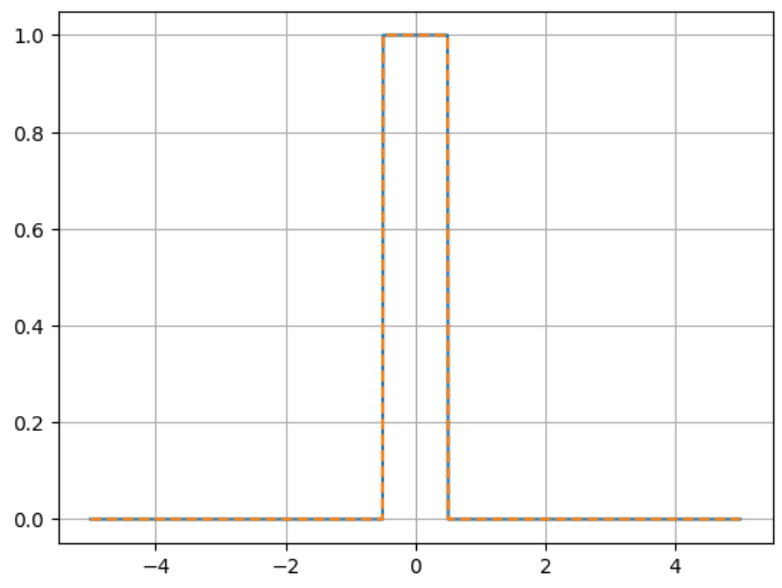
\includegraphics[width=.3\linewidth]{../image/5.jpg}   
    \caption{Исходное изображение}
\end{figure}

\noindent Переведем его в черно белый формат, поделим на $255$. Также возьмем ядро $K$:
$$
K = \begin{bmatrix}
    -1 & -1 & -1\\
    -1 & 8 & -1\\
    -1 & -1 & -1
\end{bmatrix}
$$
Двумя способами (сверткой conv2  и через образы Фурье) применим данное ядро:
\begin{figure}[!htb]
    \minipage{0.5\textwidth}
    \includegraphics[width=\linewidth]{../image/1_4_0.jpg}
    \caption{Выделение контуров сверткой} 
    \endminipage\hfill
    \minipage{0.5\textwidth}
    \includegraphics[width=\linewidth]{../image/1_4_1.jpg}   
    \caption{Выделение контуров с помощью Фурье-образа}
    \endminipage\hfill
\end{figure}

\noindent  Результаты совпали, теорема о свертки не прекразает работать.
\\ \noindent Интересно также сравнить образ Фурье исходного (*приведенного к черно-белому формату) изображения и конутра картинке, построим соответствующие образы Фурье:

\begin{figure}[!htb]
    \minipage{0.5\textwidth}
    \includegraphics[width=\linewidth]{../image/test_module_fourier_image.jpg}
    \caption{Образ Фурье исходной ч/б картинки} 
    \endminipage\hfill
    \minipage{0.5\textwidth}
    \includegraphics[width=\linewidth]{../image/test_cont_module.jpeg}   
    \caption{Фурье-образ от контура картинки}
    \endminipage\hfill
\end{figure}

\noindent Видно что центральная часть образа пропала, значит главная часть всего изображения находится именно там, в центре.
\end{document}